\documentclass{article}

\title{EE 371 Autumn 2016 - Lab 1}
\date{\today}
\author{William Li, Jun Park, Dawn Liang}

\usepackage{listings}
\usepackage{color}
\usepackage{graphicx}
\usepackage{titlesec}
\usepackage{float}

\usepackage[margin=1in]{geometry}
\usepackage[document]{ragged2e}

\titleformat{\section}{\Large\bfseries}{\thesection}{0.5em}{\uppercase}

\definecolor{dkgreen}{rgb}{0,0.6,0}
\definecolor{gray}{rgb}{0.5,0.5,0.5}
\definecolor{mauve}{rgb}{0.58,0,0.82}

\lstset{frame=tb,
  language=Verilog,
  aboveskip=3mm,
  belowskip=3mm,
  showstringspaces=false,
  columns=flexible,
  basicstyle={\small\ttfamily},
  numbers=none,
  numberstyle=\tiny\color{gray},
  keywordstyle=\color{blue},
  commentstyle=\color{dkgreen},
  stringstyle=\color{mauve},
  breaklines=true,
  breakatwhitespace=true,
  tabsize=3
}

\begin{document}

\maketitle
\newpage

\tableofcontents
\newpage

\pagenumbering{arabic}

\section{Abstract}
\paragraph{} This lab focuses on introducing us to the tools and methods of digital design. We were introduced to the various levels of abstraction in modeling and implementation, the tools involved in designing and testing hardware applications, as well as the overall design process for hardware and software and applications.

\section{Introduction}
\paragraph{} First, we built four different types of counters using different modeling techniques: a 4-bit ripple up counter using gate modeling, a 4-bit synchronous up counter using both dataflow model and schematic entry, and a 4-bit synchronous Johnson up counter using the behavioural model. In the process of building and testing these counters, we were introduced to Icarus Verilog (iVerilog) and GTKWave software, for compiling our designs and simulating waveforms. We then loaded our designs onto an Altera Cyclone V FPGA, where we verified their functionality on hardware. Then we utilised Signal Tap II, a logic analyzer for probing designs in hardware. Finally, we were briefly introduced to the C programming language. We learned the basics of a C program in the CodeBlocks IDE by compiling a provided C project, and then we built a simple C car price calculator program that asks for relevant input data and outputs an approximate list price for a brand new vehicle.

\section{Discussion}
  \subsection{Design}

  \paragraph{Design Specification} We were to build four different counters: a ripple-up counter, two synchronous up counters, and a Johnson counter, all of which counted every clock edge. Each counter used an active-low reset. The first three were directly written in Verilog, the fourth had to be built using Quartus' schematic entry feature. The ripple-up and synchronous counters count up in binary, while the Johnson counter counts up by the most significant bit.

  \paragraph{} The list price calculator was to take appropriate input data and calculate the estimated price of a new car. The program prompts the user for the manufacturer's cost, the estimated dealer's markup, the pre-tax discount, and the sales tax, and then calculates and outputs the estimated list price.

  \paragraph{Design Procedure} In Verilog HDL, we designed and implemented four counters using three different levels of modeling abstraction: structural/gate-level, dataflow, and behavioural. The first three counters were implemented using the D-flipflop provided in the lab spec; the fourth counter was implemented via Quartus' schematic entry feature, which included preset D-flipflops.

  \lstinputlisting[language=Verilog]{../counters/DFlipFlop.v}

  \paragraph{}The ripple-up counter was implemented at the structural level. The connections between the D-flipflops and outputs were explicitly assigned based on the gate-level diagram.

  \paragraph{}The first synchronous up counter was implemented at the data flow level. We diagrammed the states and generated boolean expressions using truth tables and K-maps, depicted below. We then drew the gate-level diagram from those expressions.

 % \begin{figure}
 % 	\centering
 % 	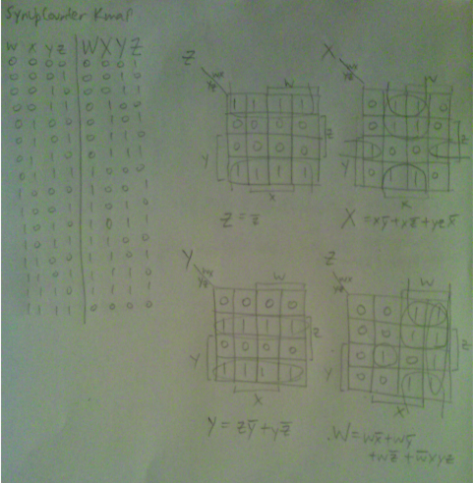
\includegraphics[width=\linewidth]{figures/synch_k_maps.png}
 % 	\caption{K-map logic reduction for synchronous counter}
 % 	\label{fig:synCounter_kmap}
 % \end{figure}

  \paragraph{}The johnson counter was implemented at the behavioural level. All behaviour was described within the verilog code. To draw our gate-level diagram, we diagrammed the states and generated boolean statements using truth tables and K-maps.

 % \begin{figure}
 % 	\centering
 % 	\includegraphics[width=\linewidth]{figures/johnson_k_maps.png}
 % 	\caption{K-map logic reduction for synchronous counter}
 % 	\label{fig:synCounter_kmap}
 % \end{figure}

  \paragraph{}The second synchronous up counter was built via schematic entry, a feature of Quartus II. The verilog code was then generated from the schematic.

  \paragraph{System Description} The four counters take a clock and reset as the input. For one of the synchronous counters, built with Quartus' schematic entry, we included an 'enable' signal input, which acts as an pause/resume switch. All four counters output 4-bits, counting up, to LEDs 3-0 of the DE1-SoC board.

  \paragraph{} The list price calculator takes the manufacturer's cost (\$), the estimated markup (\%), the pre-tax discount (\%), and sales tax (\%) as inputs. It then calculates the estimated list price of a vehicle, calculated from those values, and displays it to the user as output.

  \subsection{Test}

  \paragraph{Test Plan} The counters need to be tested to see that they count each clock edge, and reset to 0 when the active-low reset was triggered. The asynchronicity of the clock and reset signal creates the risk of metastable behaviour, which must be checked for each counter.

  \paragraph{} The listPrice calculator must be tested to see how it handle various types of inputs. Its output must be verified against external calculations to ensure it follows the correct calculations.

  \paragraph{Test Specification} The counters were both simulated on our computers and tested on the physical board. Each possible state was simulated, in regards to the reset, the 4 bits, and in the case of the schematic synchronous counter, the enable signal.

  \paragraph{} The listPrice calculator's inputs were tested against possible edge cases, such as negative values or invalid inputs like strings. Additionally, expected inputs were also tested, to verify the mathematical validity of the program.

  \paragraph{Test Cases} In simulation, the counters were connected to a clock and reset signal (in the case of the fourth counter, an additional enable signal connected). For each counter, the reset was triggered, untriggered, and then the clock ran until the reset was triggered again. The 4-bit outputs were measured to ensure appropriate counting behaviour, counting up at each clock edge and resetting to 0 when triggered.

  \paragraph{} On the board, the counters were connected to a switch for reset and four LEDs for outputs (for the fourth counter, an additional switch for enable). The reset was triggered, untriggered, then the clock ran until the reset was triggered again. The 4-bit outputs were monitored on the LEDs, and their behaviour checked to ensure they were counting up at each clock edge and resetting when triggered. In the case of the fourth counter, the enable signal was also checked to see if it paused/resumed counting.

  \paragraph{} The listPrice calculator was tested by running the program and checking edge cases. We tested regular, expected inputs, as well as negative value and string inputs, to check handling of unexpected inputs.

\section{Results}

  \paragraph{} In simulation and on the DE1-SoC board, our four counters worked as expected. They incremented by 1 bit at each clock edge, cycling back to 0 once the maximum had been reached. They reset to 0 when signaled, showing no signs of metastable behaviour. For the fourth counter, the enable signal properly paused/resumed the counter. All evidence shows that our counter designs worked.

  \paragraph{} Between the three different

  Compare and contrast the structural, dataflow, and behavioural level Quartus synthesized gate level implementations of the three counters with their gate level equivalents that you designed. Are there differences and if so, what are they and are they important? Why or why not?

  1. In the Quartus II IDE, setup and configure the Signal Tap II logic analyzer to display the inputs and outputs of each of the four counters you designed in part 1 as they are running on the DE1-SoC board. Configure the Signal Tap II to trigger on the trailing (rising) edge of the input reset signal.
2. Configure the Signal Tap II to trigger on and capture and display data following the third state in each of your counters.
3. How do the displayed signal outputs compare with the ideal signals?


  \paragraph{} Our listPrice calculator design was also successful. In the case of expected inputs, the program behaves as it should. For negative inputs, the program outputs a mathematically valid but nonsensical result (a negative price). For string inputs, the program throws an error and crashes.

\section{Analysis of Errors}

  \paragraph{}We performed failure modes and effects analysis for three counters.

  \paragraph{Ripple-up counter}

  \paragraph{Synchronous up counter} 

  \paragraph{Johnson counter}

  \paragraph{} We encountered many issues when trying to get Signal Tap II working. 

\section{Summary and Conclusion}

  \paragraph{Summary} This lab involved designing and building four 4-bit counters at various levels of abstraction in Verilog, to compare the various RTL implementations. We then tested them both in simulation and on the physical board. We also grew acquainted with iverilog and gtkwave as tools for compiling and simulating our designs, and Signal Tap II for debugging our hardware. We were then introduced to the C language, and wrote a simple program involving a few numerical inputs, calculations, and output. We were also introduced to the basic design process, involving spec writing and detailed descriptions of our project deliverables.

  \paragraph{Conclusion} Overall, the project was good for getting oriented with the environments and tools we will be using throughout the rest of the quarter. We refreshed ourselves with Quartus and verilog, and we were introduced to new tools like iverilog, gtkwave, Signal Tap II, and CodeBlocks. However, it was very messy and fragmented, and many resources were difficult to find. The spec was vague and unclear at many points, and a lot of the project was left up to our discretion.

\section{Appendix}
\subsection{Designing and Building VHDL applications - Counters}

	\subsubsection{Verilog code}

	\paragraph{Ripple-up counter} The ripple-up counter, implemented at the gate-level
	\lstinputlisting[language=Verilog]{../counters/rippleUpCounter.v}
	\lstinputlisting[language=Verilog]{../counters/rippleUpCounter_tester.v}

	\paragraph{Synchronous up counter} The synchronous up counter, implemented at the dataflow level
	\lstinputlisting[language=Verilog]{../counters/synUpCounter.v}
	\lstinputlisting[language=Verilog]{../counters/synUpCounter_tester.v}

	\paragraph{Johnson Counter} The johnson counter, implemented at the behavioural level
	\lstinputlisting[language=Verilog]{../counters/johnsonUpCounter.v}
	\lstinputlisting[language=Verilog]{../counters/johnsonUpCounter_tester.v}

	\paragraph{Synchronous up counter (schematic entry)} Schematic of the synchronous up counter, designed using Quartus' schematic entry

	\begin{figure}[H]
		\centering
		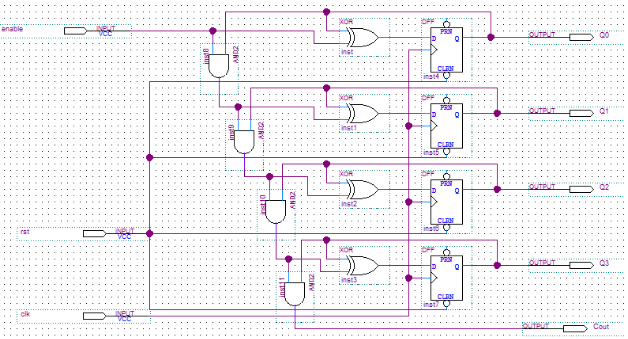
\includegraphics[width=0.75\linewidth]{figures/schem_synUp.png}
		\caption{Synchronous counter schematic entry}
		\label{fig:synUp_schem}
	\end{figure}

	\paragraph{} The generated verilog code
	\lstinputlisting[language=Verilog]{../counters/schematicEntrySynUpCounter.v}

	\subsubsection{Waveforms}
	\begin{figure}[H]
	  \centering
	  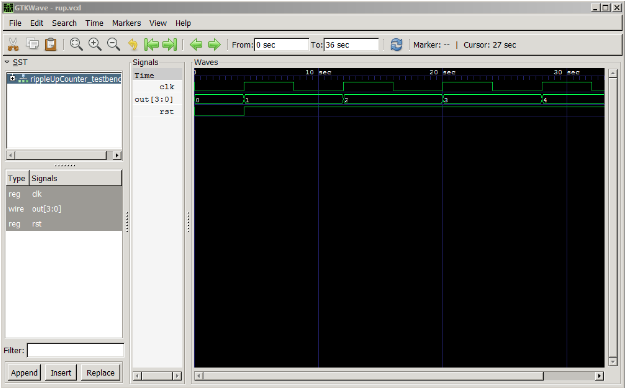
\includegraphics[width=0.75\linewidth]{figures/waveforms/rippleUp_wave.png}
	  \caption{Ripple-up counter waveform in gtkwave}
	  \label{fig:rippleUp_waveform}
	\end{figure}

	\begin{figure}[H]
	  \centering
	  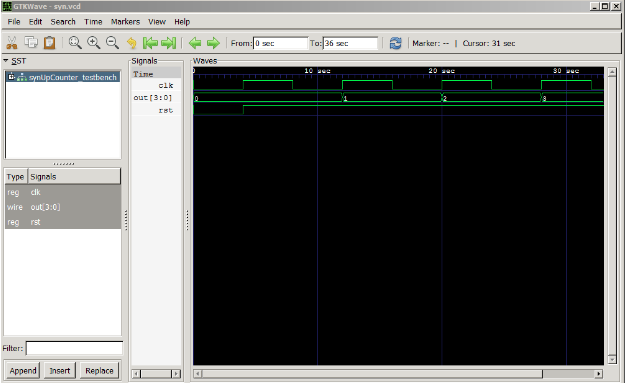
\includegraphics[width=0.75\linewidth]{figures/waveforms/synUp_wave.png}
	  \caption{Synchronous up counter waveform}
	  \label{fig:synUp_waveform}
	\end{figure}

	\begin{figure}[H]
	  \centering
	  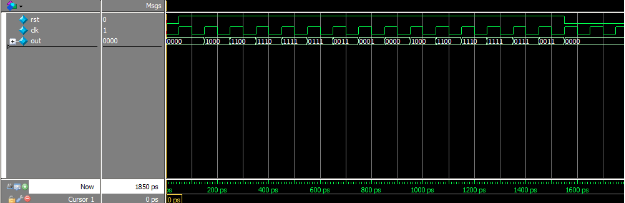
\includegraphics[width=0.75\linewidth]{figures/waveforms/johnson_wave.png}
	  \caption{Johnson counter waveform in gtkwave}
	  \label{fig:johnson_waveform}
	\end{figure}

	\begin{figure}[H]
	  \centering
	  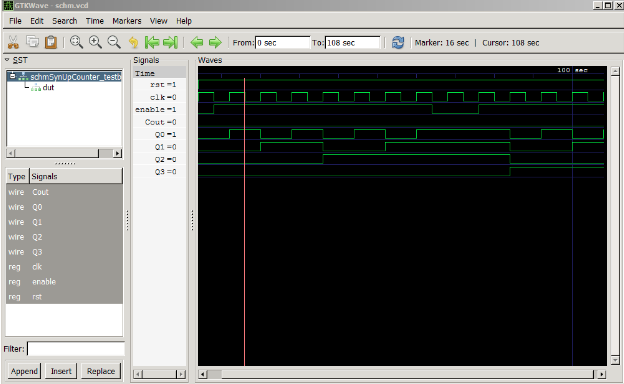
\includegraphics[width=0.75\linewidth]{figures/waveforms/schem_synUp_wave.png}
	  \caption{Synchronous up counter (schematic entry) waveform in gtkwave}
   	  \label{fig:schem_synUp_waveform}
	\end{figure}

	\subsubsection{RTL views}
	\begin{figure}[H]
	  \centering
	  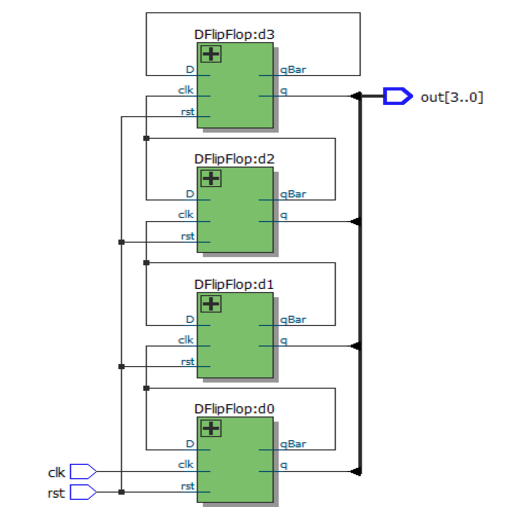
\includegraphics[width=0.75\linewidth]{figures/RTLs/rippleUp_RTL.png}
	  \caption{Ripple-up counter RTL view}
	  \label{fig:rippleUp_RTL}
	\end{figure}
	  
	\begin{figure}[H]
	  \centering
	  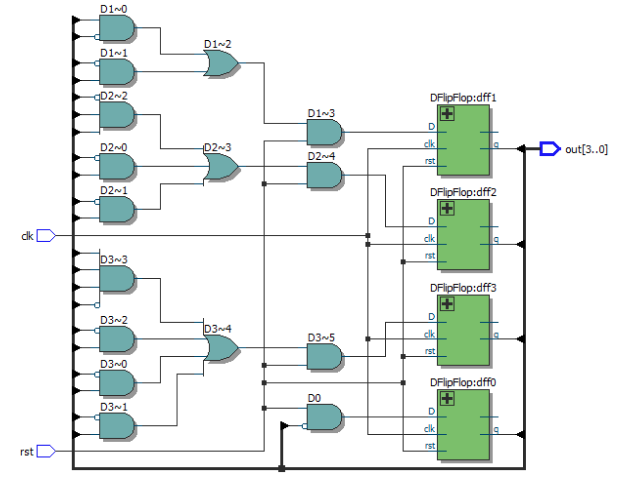
\includegraphics[width=0.75\linewidth]{figures/RTLs/synUp_RTL.png}
	  \caption{Ripple-up counter RTL view}
	  \label{fig:synUp_RTL}
	\end{figure}

	\begin{figure}[H]
	  \centering
	  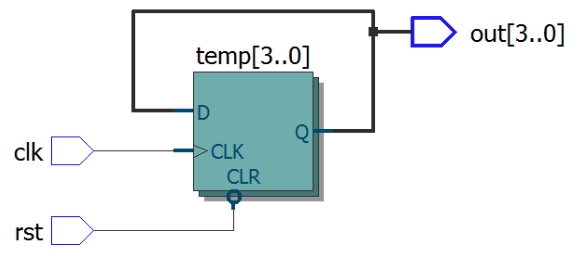
\includegraphics[width=0.75\linewidth]{figures/RTLs/johnson_RTL.png}
	  \caption{Ripple-up counter RTL view}
	  \label{fig:johnson_RTL}
	\end{figure}

	\begin{figure}[H]
	  \centering
	  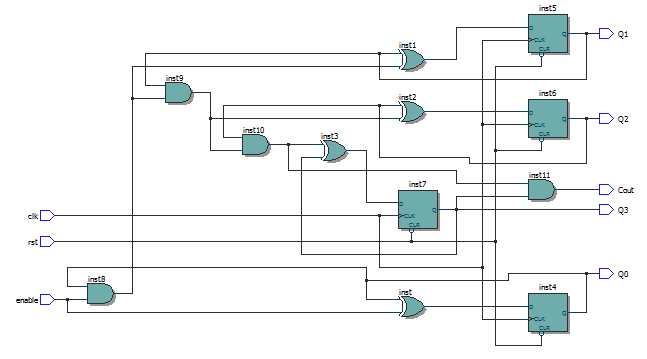
\includegraphics[width=0.75\linewidth]{figures/RTLs/schem_synUp_RTL.png}
	  \caption{Ripple-up counter RTL view}
	  \label{fig:schem_synUp_RTL}
	\end{figure}

\subsection{iverilog \& gtkwave}
	\paragraph{} We were provided verilog code to test, in order to familiarise ourselves with iverilog and gtkwave.

	\lstinputlisting[language=Verilog]{../iverilog_gtkwave/andOr0.v}
	\lstinputlisting[language=Verilog]{../iverilog_gtkwave/andorTop0.v}
	\lstinputlisting[language=Verilog]{../iverilog_gtkwave/testBench.v}

	\begin{figure}[H]
	  \centering
	  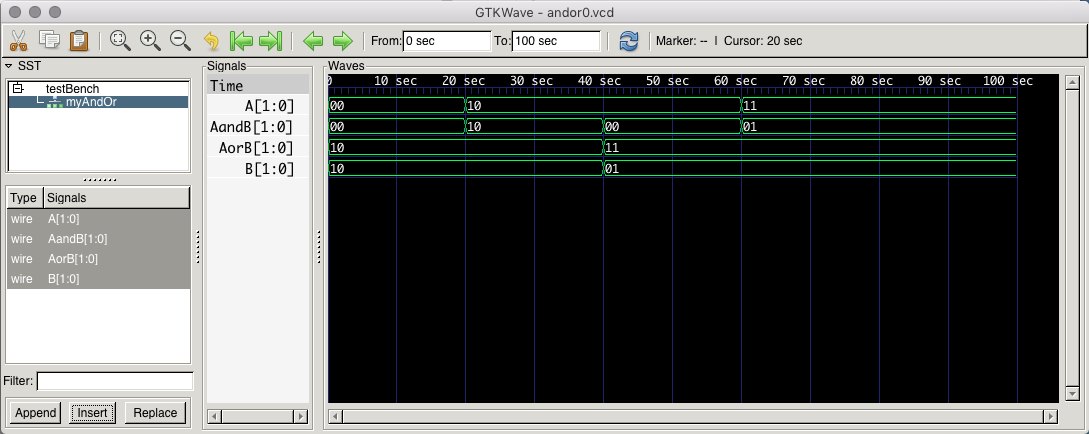
\includegraphics[width=0.75\linewidth]{figures/iverilog_gtkwave.png}
	  \caption{Results of iverilog \& gtkwave}
	  \label{fig:iverilog_gtkwave}
	\end{figure}

\subsection{Learning the C language}
\paragraph{} The car listPrice C program we wrote
\lstinputlisting[language=C]{../listPrice/listPrice.c}

\end{document}